\documentclass[a4paper, 12pt, openright, oneside, german, french, brazil, english, article]{abntex2}
\usepackage[brazil]{babel}
\usepackage{graphicx}
\usepackage[utf8]{inputenc}
\usepackage{graphicx}
\usepackage{wrapfig}
\usepackage{lscape}
\usepackage{rotating}
\usepackage{epstopdf}
\usepackage[alf]{abntex2cite}
\usepackage[a4paper, left=2cm, right=2cm, top=2cm, bottom=2cm]{geometry}
\usepackage{indentfirst}
\usepackage{longtable}
\pagestyle{plain}

%A Construção Social da Qualidade no Mercado da Música de Concerto
\titulo{The social construction of quality in Brazilian Classical Music market}
\autor{Neylson J. B. F. Crepalde (GIARS - UFMG) \and Dr. Silvio Salej Higgins (GIARS - UFMG) \and Dr. Emmanuel Lazega (CSO - SciencesPo)}
\data{October, 2017}
%\instituicao{UNIVERSIDADE FEDERAL DE MINAS GERAIS
%	\par
%	Faculdade de Filososia e Ciências Humanas}
%\local{Belo Horizonte}
%\orientador{Dr. Silvio Salej Higgins (PPGS -- UFMG)}

%\coorientador{Dr. Emmanuel Lazega (Sciences Po, CSO -- Paris)}
%\preambulo{Projeto de Pesquisa apresentado ao Programa de Pós-Graduação em Sociologia da UFMG como requisito para ingresso no Programa Doutorado Sanduíche no Exterior (PDSE).}
%\tipotrabalho{Tese (doutorado)}


\begin{document}
	\textual
	\maketitle
	
	\section{Introduction}

	%Para que o produto final por excelência de uma orquestra, a saber o concerto, venha a existir e chegue ao seu destino, o público, uma série de atores se envolvem em diversos processos de cooperação e mobilizam uma série de recursos construindo um sistema de produção em rede, ou o que Howard Becker chamaria de um ``mundo da arte'' (\textit{Art World}). Para \citeonline[p. 1, tradução do autor]{becker2008art}, ``a existência de mundos da arte, bem como o modo como sua existência afeta tanto a produção quanto o consumo de obras de arte, sugere uma abordagem sociológica para as artes'' \footnote{The existence of art worlds, as well as the way their existence affects both the production and consumption of art works, suggests a sociological approach to the arts.}.

	In order for the final product of an orchestra, the concert, come into existence e reach its destination, the public, a number of actors engage in multiple cooperation processes and mobilize multiple resources building a production network system, or what Howard Becker would call an ``Art World''. To \citeonline[p. 1]{becker2008art}, ``the existence of art worlds, as well as the way their existence affects both the production and consumption of art works, suggests a sociological approach to the arts''.
	
	%Por outro lado, se prestamos atenção à dinâmica comum aos mercados, o que percebemos com maior facilidade é um ambiente altamente concorrencial. O fenômeno supracitado é abordado por \citeonline{lazega2009theorie} de uma perspectiva distinta: no mundo concorrencial, os atores se veem constantemente em situações em que buscam a estabilidade do mercado tornando-o viável. Isso não acontece simplesmente de acordo com a lei da oferta e da demanda mas a partir do posicionamento dos produtores numa escala de qualidade que diferencia seus produtos. Para que isso seja possível, a concorrência total é inviável já que existe uma parcela de interdependência entre produtores. Essa visão está ancorada na perspectiva relacional a qual concebe mercados como estruturas sociais, empresas, Estados, etc., como estruturas em rede \cite{white2008,white2002markets,lazega2014redes}.

	On the other hand, if we pay attention to the common market dynamics, what we can perceive more easily is a highly competitive environment. The mentioned phenomenon is approached by \citeonline{lazega2009theorie} from a different perspective: in the competitive world, actors constantly see themselves in situations where they seek market's stability making it viable. This does not happen simply because of the law of supply and demand but from producers positioning in a quality scale that differentiates their products. For this to be possible, full competition is not viable since there is some interdependence between producers. This vision is anchored on the relational prespective which conceives markets as social structures and enterprises, states, etc. as network structures \cite{white2008,white2002markets,lazega2014redes}.


	%O foco deste trabalho é descortinar o mercado da música de concerto. Esse mercado ainda permanece fora do interesse convencional de economistas, sociólogos e demais estudiosos dos mercados, talvez por uma mera obra do acaso, talvez por sua alta complexidade e especificidade. Antes de apresentar nossas perguntas de pesquisa e nossos objetivos, faz-se necessário uma imersão na literatura de base realizando uma revisão tão profunda quanto possível. Após essa revisão, tentaremos extrair da observação da própria literatura (considerando o que já está postulado e, sobretudo, as lacunas existentes) os rumos de nossa investigação.
	
	The main goal of this work is to uncover the classical music market. This market still remains out of the common sense interest of economists, sociologists and other market scholars, maybe by chance, maybe by its high complexity and specificity.Before presenting our research questions and our goals, it is necessary to do an immersion in the specific literature in order to make a theoretical review as deep as possible. Afterwards, we will try to extract from the observation of the literature (considering what is already postulate and, above all, the identified gaps) the direction of our investigation.

	%Desse modo, iniciaremos o trabalho apresentado brevemente uma pesquisa bibliográfica realizada em duas das principais bases de produção acadêmica disponíveis na área de sociologia e economia. Encontramos que a produção científica sobre o mercado da música de concerto nos últimos 30 anos é ínfima. Depois, investigaremos na teoria econômica o conhecimento já sedimentado sobre bens culturais buscando entender os desafios colocados por nosso objeto de pesquisa. No terceiro capítulo, apresentaremos o framework teórico adotado para as análises, qual seja, a Análise de Redes Sociais (\textit{Social Network Analysis})\footnote{Muito embora, antecipamos, as ferramentas conhecidas como \textit{social network analysis} não constituem uma teoria geral do mundo que dedutivamente se aplique a qualquer realidade complexa. Trata-se, aqui, de um conjunto de ferramentas metodológicas aliadas a uma concepção de relações sociais.}. No quarto capítulo apresentaremos o desenho de pesquisa explicitando que tipo de dados intencionamos coletar, os procedimentos adotados, as formas de análises e os resultados esperados. Por fim, apresentamos uma investigação preliminar iniciada com uma das orquestras da cidade de Belo Horizonte bem como as considerações finais deste projeto.

	Therefore, we will begin our work presenting the results of our biliographic research. It was made in two of the main abstract bases in sociology and economics\footnote{Sociological Abstracts and Econlit.}. We found that the scientific research on music market in the last 30 years is almost nonexistent. Afterwards, we will investigate what is already settled on cultural goods seeking to understand the challenges put by our research object. In the third chapter, we will present the theoretical framework adopted for the analysis, Social Network Analysis. In the fourth chapter, we will present the research design explaining what kind of data we intend to collect, the adopted procedures, the analysis and the expected results. Finally, we present a preliminary investigation with one of the orchestras in Belo Horizonte as well as the final discussion of this project.

	%Para o autor, ``a construção coletiva da qualidade implica que a viabilidade do mercado vem do coletivo, e que é a estrutura do conjunto do mercado viável que cria a divisão de lucros\footnote{La construction collective de la qualité implique ainsi que la viabilité du marché vient du collectif, et que c'est la structure d'ensemble du marché viable qui crée le partage des rentes.}'' \cite[p. 563, tradução do autor]{lazega2009theorie}. 

	

	%Desse modo, para que esse mercado viável seja possível, é necessário que que as empresas se engajem constantemente numa combinação estável de concorrência e de cooperação. A emergência de uma estrutura a partir das próprias relações assimétricas entre eles pode criar vantagens para alguns. Para \citeonline{lazega2009theorie}, ``as relações de poder e os controles que eles exercem sobre as negociações são, portanto, cruciais nesse modelo. Sobre esse tipo de mercado, por definição, a troca não é jamais bilaterial, sempre multilateral e estratégica\footnote{Les relations de pouvoir et les contraintes qu'elles font peser sur les négociations sont donc cruciales dans ce modèle. Sur ce type de marché, par définition, l'échange n'est jamais bilatéral, toujours multilatéral et stratégique.}'' \cite[p. 563, tradução do autor]{lazega2009theorie}. Esse fenômeno é conhecido na literatura como \textit{coopetition}. A partir das perspectivas apresentadas, entramos na problemática que conduz nossa investigação.


	\section[Biliographic Investigation]{Results of the Bibliographic Investigation}
	
		
	%Com o objetivo de identificar o ``estado da arte"  no campo de pesquisas que envolvem o mercado da música e a economia da música, pesquisamos os \textit{abstracts} de trabalhos publicados na área entre 1983 e 2014 ($n=44$). Para isso, usamos as \textit{keywords} listadas na Figura \ref{chaves-busca} nos indexadores \textit{Sociological Abstracts} e \textit{Econlit}. A grande maioria dos trabalhos encontrados são artigos (86.36\%), quatro são teses de doutorado e dois são livros que foram publicados também a partir de trabalhos de doutorado. Os tipos de estudo mais encontrados na área foram estudos de caso (\textit{Case Studies}), estudos históricos e trabalhos de cunho quantitativo (cf. Tabela \ref{tipo-de-estudo}). Aqui é importante salientar que a codificação dos tipos de estudo foi feita a partir dos resumos consultados tendo como critério a sua citação expressa.
	
	In order to investigate the ``state of the art'' in the research field that involves music market and music economics, we researched abstracts of published works between 1983 and 2014 ($n = 44$). To do that, we used seven keywords\footnote{Music Market, Classical Music Market, Symphony Orchestras, Orchestra Market, Classical Music Economics, Classical Music Production and Music.} in Sociological Abstracts and Econlit. 86.36\% of the work found are research articles, four are doctoral dissertations and two are published books. Table \ref{tipo-de-estudo} lists the types of study found. Table \ref{metodos-usados} lists the research methods used.
	
	\begin{table}[ht]
		\ibgetab{
			\centering
			\caption{Type of Study}
			\label{tipo-de-estudo}
		}
		{\begin{tabular}{lr}
				\hline
				\hline
				Case Study &   6 \\ 
				Experimental Study &   2 \\ 
				Exploratory Study &   1 \\ 
				Historical Study &   6 \\ 
				Qualitative &   1 \\ 
				Quantitative &   5 \\ 
				Economic Sociology &   1 \\ 
				Institutionalist Economic Sociology &   1 \\ 
				\hline
			\end{tabular}
		}
		{\fonte{Elaborated by the authors.}}
	\end{table}
	
	\begin{table}[ht]
		\ibgetab{
			\centering
			\caption{Research Method used}
			\label{metodos-usados}
		}
		{\begin{tabular}{lr}
				\hline
				\hline
				Multivariate Regression Analysis &   1 \\ 
				Big Data &   1 \\ 
				Big Data + Word Count &   1 \\ 
				Comparative Analysis &   1 \\ 
				Comparative Historical Analysis &   1 \\ 
				Discourse Analysis &   1 \\ 
				Economic Method &   1 \\ 
				Field Theory / Organizational Theory &   1 \\ 
				Documental Research &   1 \\ 
				Rationalization &   1 \\ 
				Social Network Analysis &   3 \\ 
				Survey &   1 \\ 
				Web-based Experiment &   2 \\ 
				Interviews + Documentation Analysis + Statistics  &  1 \\
				Interviews + Music Journals + Promotional Literature &   1 \\ 
				\hline
			\end{tabular}
		}
		{\fonte{Elaborated by the author.}}
	\end{table}
	
	%Os temas de investigação aparecem nos trabalhos de uma maneira bastante difusa. Encontramos algumas publicações abordando aspectos culturais que influenciam o mercado da música, o mercado de trabalho dos músicos, as relações de gênero e a divisão do trabalho, financiamento e ``patronagem", o consumo da música e as variáveis que o explicam, gosto musical, padrões estéticos, identidade cultural e música nacional/folclórica, história social dos músicos, o ``cânon" do repertório musical, liderança do maestro e participação e satisfação dos músicos, música antiga\footnote{No campo da música, convencionou-se chamar de música antiga aquela escrita até o séc. XVII.}, revolução digital e indústria fonográfica.

	The investigation themes appear on the revised works on a very diffuse way. We found some publications approaching cultural aspects that influence music market, musicians labor market, gender relations and labor division, financing and patronage, music consumption and the variable that explain it, musical taste, aesthetic standards, cultural identity and national/folk music, social history of musicians, the musical repertoire canon,  conductor's leadership and participation/satisfaction of musicians, ancient music, digital revolution and music industry.

	


	\section{Os produtos culturais}
	
	%O primeiro desafio deste trabalho reside no fato de que estamos lidando com um objeto que desafia a maioria dos pressupostos da teoria econômica vigente. Comecemos, portanto, estabelecendo algumas diferenças fundamentais entre os bens culturais e as mercadorias comuns conforme concebidos tradicionalmente pela teoria econômica. Segundo \citeonline{tolila2007cultura}, as mercadorias são entendidas por meio de quatro critérios objetivos, a saber, suas propriedades físicas (as quais, nesse caso, estão diretamente relacionadas com a qualidade do produto em questão), a data e o local em que ele está disponível e aquilo que condiciona sua entrega num universo certo, i.e., sem incertezas. A qualidade de um bem, nessa perspectiva, pode ser decomposta em uma série de elementos objetivos, i.e., claramente mensuráveis e hierarquizáveis. Além disso, na teoria econômica clássica todo bem é considerado um ``bem privado'' e, portanto, ``exclusivo e rival'' no consumo. Para citar um exemplo, ``um café, um sanduíche, uma camisa, um par de sapatos, uma cadeira, etc., são bens exclusivos porque é possível impedir-me de obtê-los (\ldots); por outro lado, cada um desses bens é de consumo exclusivo porque no momento em que o aproveito, nenhuma outra pessoa pode usufruí-lo'' \cite[p. 29]{tolila2007cultura}. Ora, os produtos culturais, de um modo geral, são não exclusivos; pode-se, por exemplo, admirar um belo edifício histórico na rua sem ter que pagar por isso. Tampouco são rivais no consumo; o prazer de assistir um concerto não é diminuído pela presença de outras pessoas no público.
	
	Our fisrt challenge lies in the fact that we are dealing with an object that defies the majority of economic theory assumptions. Let us begin establishing some fundamental differences between common goods and cultural goods. According to \citeonline{tolila2007cultura}, goods are understood by four objective criteria, namely, its physical properties (which, in this case are directly related to the quality of the product), date and local where it is available and what conditions its delivery in a certain universe, i.e., without uncertainties. The quality of a good, in this perspective, can be decomposed in a bunge of objective elements, i.e., clearly measurable e hierarchical. Moreover, in neoclassical economic theory every good is considered a ``private good'' and, therefore, ``exclusive and rival'' in consumption. To cite an example, ``a coffee, a sandwich, a shirt, a pair of shoes, a chair, etc., are exclusive because it is possible to stop me from getting them (\ldots); on the other hand, each of these goods is exclusive because in the moment I enjoy it, no other person can enjoy it as well'' \cite[p. 29]{tolila2007cultura}. Cultural products in general are not exclusive; one can, for instance, admire a beautiful historic building without having to pay for it. Neither they are rivals in consumption; the pleasure of attending a concert is not diminished by the presence of other people. 

	%Esse setor da economia define-se, ainda, pela sua lógica de oferta voltada à produção, ao contrário dos mercados de bens comuns voltados ao consumo. Para \citeonline[p. 32]{tolila2007cultura}, ``essa lógica da oferta caracteriza bem, entre outras, a ação das políticas públicas em termos de investimento, de ajuda e de sustentação das atividades culturais, do patrimônio ao espetáculo ao vivo, e em termos de incentivos às práticas culturais''. De fato, os Estados e coletividades públicas tem demonstrado interesse crescente no setor cultural, o que pode ser verificado através das políticas públicas, das administrações especializadas, da alocação de recursos dirigidos especificamente ao setor e do surgimento de toda uma rede de instituições e profissionais atuantes no setor cultural, grande parte deles financiados por dinheiro público \cite{tolila2007cultura}. Para \citeauthoronline{tolila2007cultura}
	
	This sector of the economy is defined by its logic towards production, unlike market of consumer goods. States and public collectives has shown growing interest on cultural industry, what can be verified by policy making, by specialized administrations, allocation of resources directed specifically to this sector and the emergence of a whole network of institutions and professionals acting in this sector, most of them financed by public resources \cite{tolila2007cultura}.


	%\begin{citacao}
	%	Consequentemente, a atenção das autoridades, dos cidadãos e de seus representantes, foi desenvolvida em duas direções clássicas no contexto das democracias: por um lado, \textbf{o debate público interno} sobre a alocação dos recursos, o valor deles e seu significado, por outro, \textbf{a competição exterior} com os outros Estados pelas questões de mercados e de comércio. Essa segunda direção (\ldots) é inseparável dos dilemas e debates que movimentam atualmente todas as reflexões sobre \textbf{a globalização e a diversidade das expressões culturais}. \cite[p. 71-2]{tolila2007cultura}
	%\end{citacao}

	%Para esse autor, esses dois elementos são constitutivos do valor simbólico atribuído às práticas e ao desenvolvimento cultural à medida que traz relevância ao debate relacionado à identidade e diversidade cultural. O valor simbólico dos bens culturais constitui, para nós, um elemento central na compreensão de nosso objeto de estudo, muito embora, contrariando novamente a teoria econômica clássica, não seja objetivo em sua natureza mas relacional e individual, i.e., só existe à medida que é reconhecido pelo indivíduo no momento de seu consumo. Para que o valor simbólico de um determinado bem seja reconhecido, é necessário que haja estruturas cognitivas apropriadas para a compreensão e fruição do bem, ou seja, esquemas mentais adquiridos por meio da educação artística prévia \cite{bourdieu2003amor}.
	
	%As performances musicais possuem ainda uma particularidade quanto à natureza de sua existência na qual reside grande parte das dificuldades metodológicas que as cercam. \citeonline{tolila2007cultura} explica:
	
		%\begin{citacao}
	%	O que é a música? A partitura escrita? Não. Os músicos que formam a orquestra? Não. O regente? Também não. Na verdade, é quase impossível definir a música como uma ``coisa'' (uma mesa, uma cadeira, uma casa, etc.) pois ela só existe de fato no momento em que é ouvida, isto é, em uma relação com o ouvinte\footnote{Para o autor, ``na verdade, no mundo social, o modo real de existência da maioria dos fenômenos é o da relação entre seres humanos'' \cite[p. 110]{tolila2007cultura}. Curiosamente, nessa premissa se baseia todo o paradigma neoestrutural na sociologia conhecido também como ``perspectiva relacional'' ou ``teoria das redes sociais''.}. \cite[p. 109]{tolila2007cultura}
	%\end{citacao}
		
	Musical performances have also another peculiarity regarding the nature of its existence in which resides a large part of the methodological difficulties that surround them. \citeonline{tolila2007cultura} explains it: ``What is music? The score? No. The orchestra musicians? No. The conductor? Neither. In fact, it is almost impossible to define music as a ``thing'' because it only exists in fact in the very moment it is heard, that is, in a relation with the listener`` \cite[p. 109]{tolila2007cultura}.
	
		
	
	%Desse modo, a música (bem como a dança e o teatro, por exemplo) assume um modo especial de existência que envolve a participação de todos os elementos ou atores supracitados, a saber, partitura, músicos, regente, etc., na construção de sua materialidade que só existe (e portanto só é possível de ser consumida) no momento da escuta. Segundo \citeonline[p. 54]{benhamou2007economia} ``a concorrência assume a forma paradoxal de uma competição entre instituições que oferecem bens únicos e efêmeros'' onde o comportamento dos atores econômicos tende a monopólios discriminatórios. Para essa autora, o setor é caracterizado por uma fragilidade constante devido a elevações periódicas de custos e à quase-ausência de reservas de produtividade. De fato, como veremos, o paradigma vigente, no que tange a teoria econômica das performances ao vivo, aponta para um inevitável estado deficitário.

	Thus, music (as well as dance and theater) assumes a special mode of existence that involves the participation of all the elements of actors mentioned, that is, the score, the musicians, the conductor, etc., in the construction of its materiality which only exists (and can only be consumed) in the listening moment. According to \citeonline[p. 54]{benhamou2007economia}, ``competition takes a paradoxical form of a competition between institutions the offer unique and ehpemeral goods'' where economic actors behavior tend to discriminatory monopolies. To the author, the sector is characterized by a constant fragility because of periodic cost elevations and the almost absence of productivity reserves. In fact, as we will see, the current paradigm, regarding the economic theory of live performances, points to an inevitable deficit state.

	
	\section{Baumol and Bowen's model -- The Cost Disease}
	
	%William Baumol e William Bowen empreenderam, sob encomenda da Fundação Ford em 1965, uma pesquisa visando diagnosticar a situação econômica dos teatros da Broadway \cite{benhamou2007economia}. Seus achados são até hoje considerado válidos. Para \apudonline{baumol1966performing}{benhamou2007economia} a economia divide-se em dois setores, o setor 1 (arcaico) e o setor 2 (progressista). O setor arcaico não apresenta possibilidades de gerar ganhos de produtividade enquanto o setor progressista gera ganhos de produtividade a partir de inovações, de economias de escala e da acumulação de capital. A performance ao vivo faz parte do setor arcaico e isso se deve à posição que nele ocupa o trabalho.

	Baumol and Bowen did, under Ford Foundation demand in 1965, a research aiming to diagnose the economic situation of Broadway theaters \cite{benhamou2007economia}. Their findings are considered valid to this day. To \apudonline{baumol1966performing}{benhamou2007economia} economy is divided in two sector, (1) archaic and (2) progressive. Archaic sector does not have the possibility of generating productivity gains while progressive sector generates productivity gains from innovations, from scale economy and accumulation of capital. Live performanceis part of the archaic sector because of the position that work has on it.


		%O modelo de \apudonline{baumol1966performing}{benhamou2007economia} baseia-se nas três hipóteses que se seguem:
		
		Baumol and Bowen's model is based on three hypotheses:
	
	\begin{enumerate}
		%\item A economia divide-se em dois setores, arcaico e progressista. No setor arcaico, onde reside a performance ao vivo, a produtividade do trabalho é constante ou aumenta pouco e a quantidade de trabalho não pode ser diminuída sem desnaturar o produto. Sendo $L_{1,t}$ o volume de trabalho empregado no setor 1 no momento \textit{t} e \textit{a} um valor constante, a quantidade de produto no setor 1 no momento \textit{t} ($Y_{1,t}$) é obtida por $$Y_{1,t} = aL_{1,t}$$
		
		\item Economy is divided in two sectors, archaic and progressive. In archaic sector, where live performance lies, work productivity is constant or has little increases and the amount of work cannot be diminished without denaturing the product. Be $L_{1,t}$ the volume of work employed in archaic sector in moment \textit{t} and \textit{a} a constant value, the quantity of product in the archaic sector in moment \textit{t} ($Y_{1,t}$) is obtained by $$Y_{1,t} = aL_{1,t}$$.
		
		%Sejam $Y_{2,t}$ e $L_{2,t}$ respectivamente a quantidade de produto do setor progressista no momento \textit{t} e o volume de trabalho empregado no setor 2 no momento \textit{t}, seja r a taxa de aumento da produtividade do trabalho e \textit{b} uma constante, a quantidade de produto no setor é obtido por $$Y_{2,t} = bL_{2,t}[1+r]^t $$
		
		Be $Y_{2,t}$ and $L_{2,t}$ respectively the quantity of product in the progressive sector in moment \textit{t} and the amount of work employed on progressive sector in moment \textit{t}, be r the rate of increase in labor productivity and \textit{b} a constant, the quantity of product in the progressive sector is obtained by $$Y_{2,t} = bL_{2,t}[1+r]^t $$
		
		%\item Os custos de produção, comparados somente com os custos salariais (\textit{W}), evoluem no mesmo ritmo e sentido que a produtividade no setor progressista, isto é, $W_{1,t} = W_{2,t} = W_t = W[1+r]^t$. Os custos relativos de cada setor são, portanto, dados por
		
		\item Production costs, compared only to wage costs (\textit{W}), evolve in the same pace and direction that productivity in the progressive sextor, that is, $W_{1,t} = W_{2,t} = W_t = W[1+r]^t$. The relative costs of each sector are, therefore, given by
		
		$$C_1 = \frac{W_tL_{1,t}}{Y_{1,t}} = \frac{W(1+r)^tL_{1,t}}{aL_{1,t}} = \frac{W(1+r)^t}{a}$$
		$$C_2 = \frac{W_tL_{2,t}}{Y_{2,t}} = \frac{W(1+r)^tL_{2,t}}{bL_{2,t}(1+r)^t} = \frac{W}{b}$$
		
		%Tem-se, então, que o custo por unidade de produto obtido aumenta indefinidamente no setor 1 e mantém-se constante no setor 2. As funções de custos de produção em ambos os setores está representada na Figura \ref{custos-de-producao}.
		
		Thus, the cost by unit of product obtained raises indefinitely in the archaic sector and remains constant in the progressive sector. Production cost functions in both sectors is represented in Figure \ref{custos-de-producao}.
		
		% Inserir a figura plotando as duas funções
		\begin{figure}[!h]
			\centering
			\caption{Custos de Produção}
			\label{custos-de-producao}
			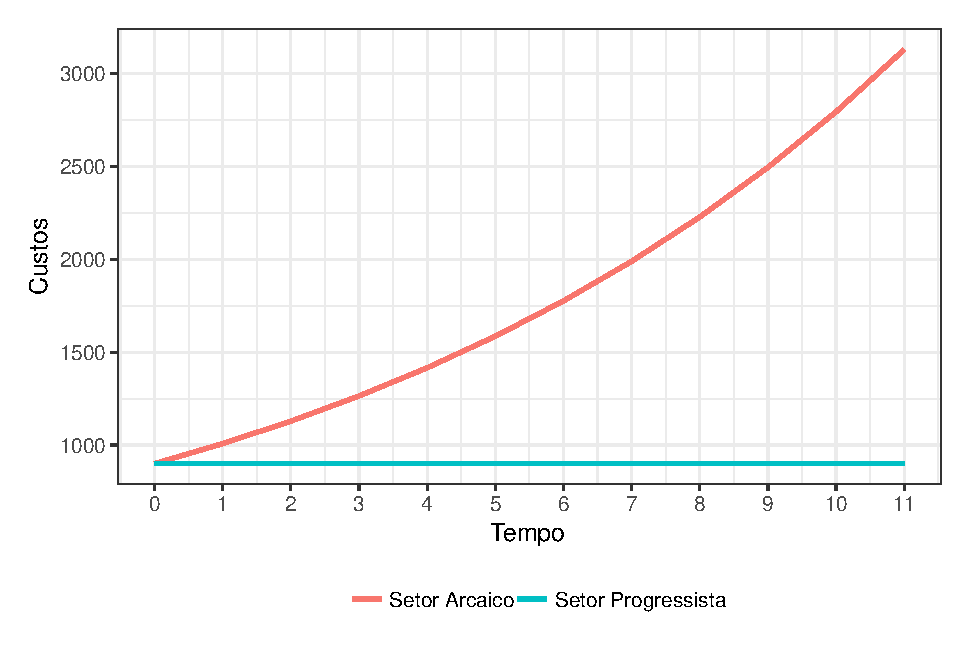
\includegraphics[scale=1]{doenca_dos_custos.eps}
			\fonte{Elaboração do autor.}
		\end{figure}
		
		
		%\item ``A demanda de espetáculos ao vivo é elástica; toda alta de preço redunda numa redução do público'' \cite[p. 56]{benhamou2007economia}. Sendo os preços proporcionais aos custos relativos nos dois setores, $P_1 = \alpha C_1$ e $P_2 = \beta C_2$, então
		
		\item ``The demand of live shows is elastic; any price increase leads to a public reduction'' \cite[p. 56]{benhamou2007economia}. If the prices are proportional to the relative costs in both sectors, $P_1 = \alpha C_1$ and $P_2 = \beta C_2$, then
		
		$$\frac{P_1Y_1}{P_2Y_2} = \frac{\alpha C_1Y_1}{\beta C_2Y_2} = Cte$$ or
		$$\frac{C_1Y_1}{C_2Y_2} = \frac{W(1+r)^t \cdot L_{1,t}}{W(1+r)^t \cdot L_{2,t}} = \frac{L_{1,t}}{L_{2,t}} = K_0$$ and
		$$\frac{Y_1}{Y_2} = \frac{aL_{1,t}}{bL_{2,t}(1+r)^t} = \frac{aK_0}{b(1+r)^t}$$
		
		%``Quando \textit{t} aumenta, $\frac{Y_1}{Y_2}$ diminui, e quando $t \rightarrow \infty$, $\frac{Y_1}{Y_2} \rightarrow 0$'' \cite[p. 57]{benhamou2007economia}. Desse modo, a produção do setor arcaico (1) diminui fatalmente.
	%\end{enumerate}
	
	``When \textit{t} increases, $\frac{Y_1}{Y_2}$ decreases and when $t \rightarrow \infty$, $\frac{Y_1}{Y_2} \rightarrow 0$'' \cite[p. 57]{benhamou2007economia}. Thus, production in the archaic sector fatally descreases.
	
	\end{enumerate}
	%De forma complementar à lei de Baumol, \citeonline{throsby1994production} desenvolve uma função da produção do espetáculo ao vivo a qual pode ser sintetizada da seguinte forma:
	
	Complementarily to Baumol's law, \citeonline{throsby1994production} develops a function of live performance production which can be synthesized in this way:
	
	%O número de representações de uma determinada temporada deve ser fixado levando em conta a capacidade da sala \textit{v}. Sejam $L^s$ e $K^s$ o trabalho e o capital necessários para montar uma produção, sejam $L^r$ e $K^r$ o trabalho e o capital requeridos por cada representação da produção, o número de espectadores da iésima representação da jésima produção, $y_{ij}$, tal que $y_{ij} \leq v$, é dado por
	
	The number os presentations in a given season must be fixed taking into account the capacity of the auditorium \textit{v}. Be $L^s$ and $K^s$ the necessary work and capital to a production, be $L^r$ and $K^r$ the work and capital required by each performance of the production, the number of spectators of the performance \textit{i} of the production \textit{j}, $y_{ij}$, such that $y_{ij} \leq v$, is given by
	$$y_j = \sum_iy_{ij} = y_i(L^{s}_{j}, K^{s}_{j}, m_j, q_j) $$ where
	%o número de representações da jésima produção $$m_j = m_j(L^{r}_{j}, K^{r}_{j})$$ e $q_j$ resume as qualidades da jésima produção as quais, nesse contexto, podem ser medidas pela luxuosidade (\textit{lavishness}) da produção. Nesse caso, $q_j$ não é independente de $L^s$ e $K^s$. Espera-se que $$\frac{\partial y_j}{\partial m_j} > 0 \quad, \quad \frac{\partial^2y_j}{\partial m^{2}_{j}} < 0,$$ isto é, extender a temporada pode reduzir o número de espectadores na margem.
	
	the number of performances of the production \textit{j} $$m_j = m_j(L^{r}_{j}, K^{r}_{j})$$ and $q_j$ summarizes the qualities of the production \textit{j} which, in this context, can be measured by the lavishness of the production. In this case, $q_j$ is not independent of $L^s$ and $K^s$. It is expected that $$\frac{\partial y_j}{\partial m_j} > 0 \quad, \quad \frac{\partial^2y_j}{\partial m^{2}_{j}} < 0,$$ that is, extend the season can decrease the spectators number in the margin.
	
	%Segundo \citeonline[p. 59]{benhamou2007economia} ``a conclusão do modelo [de Baumol] é a inelutabilidade do aumento dos déficits dos espetáculos ao vivo''. Esse modelo tem sido corroborado por várias pesquisas \cite[e.g.]{throsby1979economics,leroy1980economie,peacock1983inflation,baumol1984inflation,dias2011artes} e, para \citeonline[p. 54]{benhamou2007economia}, essa característica do setor é suficiente para justificar o aumento das subvenções públicas e da prática do mecenato mesmo tendo em vista que ``essa intervenção maciça, distribuída de forma muito desigual, não é suficiente para garantir ao setor um equilíbrio financeiro duradouro''. Para \apudonline[p. 320]{baumol1966performing}{luksetich2011orchestras}, ``se se concorda que a artes de performance conferem benefícios gerais à comunidade como um todo\ldots as artes são bens públicos cujos benefícios demonstravelmente excedem as receitas que se espera coletar na bilheteria\footnote{If one agrees that the performing arts confer general benefits on the community as a whole\ldots the arts are public goods whose benefits demonstrably exceed the receipts one can hope to collect at the box office.}''. O modelo, entretanto, possui inconsistências, algumas delas apontadas por \citeonline{benhamou2007economia}.
	
	According to \citeonline[p. 59]{benhamou2007economia} ``the conclusion of Baumol's model is the ineluctability of the increase on deficit of live performance''. This model has been corroborated by many researches \cite[e.g.]{throsby1979economics,leroy1980economie,peacock1983inflation,baumol1984inflation,dias2011artes} and, to \citeonline[p. 54]{benhamou2007economia}, this sector characteristic is suficient to justify the increase of public subsidies and the practice of patronage even in view of the fact that ``this massive intervention, distributed in a very unequal way, is not enough to ensure to the sector a lasting financial equilibrium''. To \apudonline[p. 320]{baumol1966performing}{luksetich2011orchestras}, ``if one agrees that the performing arts confer general benefits on the community as a whole\ldots the arts are public goods whose benefits demonstrably exceed the receipts one can hope to collect at the box office''. 
	
	%%% Será que eu continuo este pedaço aqui????????????????
	
	%The model, however, has inconsistencies, some of them pointed by \citeonline{benhamou2007economia}.
	
	%A primeira consiste do pressuposto de que os salários do setor 1 são iguais aos do setor 2. Entretanto, desde a Segunda Guerra Mundial, os salários médios no setor do espetáculo ao vivo apresentaram uma tendência a crescerem menos do que no outro setor \apud{throsby1994production}{benhamou2007economia}. A segunda consiste do pressuposto altamente discutível de que a demanda é sensível ao preço. Maior parece ser o efeito da qualidade (percebida) do espetáculo sobre a demanda. De fato, \citeonline{throsby1994production} salienta que, por causa da dificuldade na medição da qualidade das performances, os efeitos dessa variável usualmente ficam restritos ao termo do erro nos modelos econométricos com a exceção de um estudo experimental conduzido pelo próprio \citeonline{throsby1983quality}. Nesse trabalho, o autor identificou algumas características da qualidade da performance no teatro como a qualidade da atuação, da produção, do roteiro e encontrou que a demanda é inelástica com relação ao preço dos ingressos mas \textit{altamente correlacionada com a qualidade esperada}. Este ponto parece central na investigação do mercado das orquestras e será desenvolvido oportunamente.
	
	
	
	%Além disso, é possível reduzir os custos de uma produção de espetáculo ao vivo de várias formas, a saber, através da gravação e reprodução do espetáculo, através do uso, na música, de sons \textit{sampleados} ou eletrônicos ao invés da contratação de músicos, a utilização de um mesmo ator representando mais de um papel em uma montagem cênica ou a reutilização de cenários e figurinos (práticas comum em montagens modernas de ópera), dentre várias outras. Para \citeonline[p. 60]{benhamou2007economia} esses meios ``equivalem a substituir o déficit comercial por um `déficit artístico'. Mesmo assim, essas medidas não são suficientes para compensar a diferença de produtividade. 
	
	%A terceira inconsistência reside no fato de que a alta da produtividade nos setores progressistas acompanhada por um aumento de salário proporcional à melhora das qualificações provoca um crescimento da procura por espetáculos, o que \textit{per se} contribui com a solução das dificuldades criadas pela diferença de produtividade nos setores \apud{throsby1979economics}{benhamou2007economia}. O crescimento, para \apudonline{baumol1966performing}{benhamou2007economia} reside na presença de consumidores cada vez mais sagazes e exigentes e acaba por gerar custos marginais superiores às receitas. ``As companhias musicais ajudaram a construir a reputação de artistas cuja contratação se tornou inevitável. A consequência é um aumento exagerado dos cachês e dos custos'' \cite[p. 61]{benhamou2007economia}. 
	
	%Por mais que seja verdadeira esta última constatação sobre os custos gerados na contratação de artistas de renome, parece também uma grande ingenuidade acreditar que o aumento de salário acarreta um crescimento na procura por espetáculos ao vivo. Na verdade os estudos em sociologia econômica tem mostrado, como veremos, que o consumo artístico está ligado ao que Bourdieu (\citeyear{bourdieu2011forms,bourdieu2003amor,bourdieu2007distincao}) chama de ``capital cultural'' e à construção de uma identidade social. 
	
	%A quarta inconsistência é esta: A gravação dos espetáculos pode gerar receita. Embora as rendas de espetáculos gravados sejam pequenas conforme investigações no contexto americano \apud{heilbrun2001economics}{benhamou2007economia} parecem ser um recurso bastante explorado no setor Algumas orquestras brasileiras costumam disponibilizar as gravações de seus concertos e óperas como produto secundário da sua carta de produtos. Gravações de estúdio e ainda outros produtos (camisetas, acessórios, \textit{souvenirs}) compõem o financiamento dessas instituições. Oportunamente abordaremos esse ponto.
	
	%\citeonline{throsby1994production}, após revisar vários estudos que testam a lei de Baumol conclui que
	
	%\begin{citacao}
		%Os impactos combinados dos ajustes de produção aumentaram a demanda e níveis crescentes de receita não esperada contrariaram qualquer tendência em direção a um aumento secular nos déficits entre companias de performance sugerindo que, embora a doença dos custos irá indubitavelmente continuar a presentear a artes performáticas com problemas difíceis, é improvável que chegue ao extremo\footnote{the combined impacts of production adjustments increased demand, and generally rising levels of unearned revenue have countered any tendency towards a secular rise in deficits among performance companies, suggesting that although the cost disease will doubtless continue to present the performing arts with difficult problems, it is unlikely to be terminal.}. \cite[p. 16]{throsby1994production}
	%\end{citacao}
	
	%Por fim, a análise de \citeonline{baumol1966performing} apontando a especificidade do setor contribuiu tanto para o desenvolvimento do programa de pesquisa que hoje conhecemos como economia da cultura quanto para o reconhecimento da necessidade de vinculação dos espetáculos ao vivo à esfera não-comercial subvencionada. Sigamos agora examinando como o mercado cultural brasileiro obtém seus recursos e o principal mecanismo de financiamento para que isso aconteça: as leis de incentivo à cultura.
	
	Baumol's analysis pointing the specificities of the sector contributed to both the development of the research program that we know today as economy of culture and the recognition of the necessity of binding live performances to the subsidized non-commercial sphere. Let us continue examining how brazilian cultural market obtains its resources and its main financing mechanism, the laws to encourage culture.

	\subsection{The laws to encourage culture}
	
	\ldots


























	This research project aims to look into the market of classical music in the Southeast region of Brazil. The research is guided by two main questions: 1) Understanding that the orchestras' market does not operate as an usual market, how does it work?;  who are the actors involved and which are the actions that each one develops within the system? 2) Which are the conditions and social factors of the production of orchestral music quality standards, i.e., how this quality standard to which everyone is commited to is produced and sustained?
	
%	Este trabalho visa debruçar-se sobre o mercado da música de concerto na região Sudeste do Brasil. A investigação é norteada por duas principais perguntas: 1) Entendendo que o mercado das orquestras não opera como um mercado comum, como se dá seu funcionamento; quem são os atores envolvidos e quais são as ações que cada um desenvolve no sistema? 2)Quais são as condições e fatores sociais de produção de padrões de qualidade da música de concerto, ou seja, como é produzido e mantido o \textit{standard} de qualidade com o qual todos estão comprometidos?

	To develop our study, it is necessary to transcend the limits with which the economic theory encountered when addressing cultural products. In all it's history, economic theory has anchored his main discoveries in two assumptions. The first leads to the idea of \textit{homo economicus}, i.e., the rational actor who makes decisions aiming to boost profits and reduce losses. To do that, he has access to complete information and he is capable of processing them entirely. This assumption gives the economy the capacity of elaborating elegant models to explain people's choices and preferences but cannot incorporate a central part of social life: culture. Economic sociology has develop itself mainly addressing the gaps left by this assumption seeking to give account for how social norms, values, status systems and prestige influence economic action. Put another way, a sociological perspective makes possible to see relational factors that help to answer classical questions of economy while it brings the studies closer to reality even if it does not have such elegant models or such consistent logic \cite{hirsch1987dirty}. Economic sociology is worried with contextual elements of economic trades, i.e., to analyze how interactions between actors bring out a market and how this interactions regulate and control the markets.

	
%	Para desenvolvermos nosso estudo faz-se necessário transcender os limites com os quais a teoria econômica se deparou ao abordar produtos culturais. Ora, em todo o seu decurso, a teoria econômica tem ancorado seus principais achados em dois pressupostos. O primeiro remonta à ideia do \textit{homo economicus}, ou seja, o ator racional que toma decisões visando potencializar ganhos e diminuir perdas. Para isso, ele tem acesso à completude das informações de que precisa e é capaz de processá-las inteiramente. Esse pressuposto dá à economia a capacidade de elaborar modelos elegantes para explicar escolhas e preferências mas não consegue incorporar uma parte central da vida social, a saber, a cultura. A área da sociologia econômica desenvolveu-se, sobretudo, se debruçando sobre as lacunas deixadas por esse pressuposto buscando dar conta de como normas sociais, valores, sistemas de status e prestígio influenciam a ação econômica. Dito de outra forma, uma perspectiva sociológica possibilita enxergar fatores relacionais que ajudam a responder a perguntas clássicas da economia além de tornar o estudo mais próximo da realidade mesmo não tendo modelos tão elegantes e nem lógica tão consistente \cite{hirsch1987dirty}. A sociologia econômica está preocupada com elementos contextuais das trocas econômicas, ou seja, analisar como as interações entre os atores fazem emergir um mercado e como essas interações regulam e controlam os mercados.
	
	The second assumption is the general characterization of market products. The products are understood by four objective criteria, namely, their physical properties (which in this case are directly related to the quality of the concerned product), the date and the place where they are available and what determines their delivery within a certain universe, i.e., without uncertainties. The quality of a product, in this view, can be decomposed into a series of objective elements, i.e., clearly measurable and ordered. Moreover, in classical economic theory every good is considered a `` private good '' and therefore ``unique and rival'' in its consumption. To give an example, ``a cup of coffee, a sandwich, a shirt, a pair of shoes, a chair, etc., are exclusive property because you can prevent me to get them (\ldots); on the other hand, each of these goods is for exclusive consumption because in the moment that I enjoy it, no one else can enjoy it'' \cite[p. 29]{tolila2007cultura}. However, the cultural products, generally, are not unique; You can, for example, admire a beautiful historic building on the street without having to pay for it. Nor they are rival in consumption; the pleasure of attending a concert is not diminished by the presence of other people in the audience.
	
	
%	O segundo pressuposto consiste da caracterização geral dos produtos mercantis. As mercadorias são entendidas por meio de quatro critérios objetivos, a saber, suas propriedades físicas (as quais, nesse caso, estão diretamente relacionadas com a qualidade do produto em questão), a data e o local em que estão disponíveis e aquilo que condiciona sua entrega num universo certo, i.e., sem incertezas. A qualidade de um bem, nessa perspectiva, pode ser decomposta em uma série de elementos objetivos, i.e., claramente mensuráveis e hierarquizáveis. Além disso, na teoria econômica clássica todo bem é considerado um ``bem privado'' e, portanto, ``exclusivo e rival'' no consumo. Para citar um exemplo, ``um café, um sanduíche, uma camisa, um par de sapatos, uma cadeira, etc., são bens exclusivos porque é possível impedir-me de obtê-los (\ldots); por outro lado, cada um desses bens é de consumo exclusivo porque no momento em que o aproveito, nenhuma outra pessoa pode usufruí-lo'' \cite[p. 29]{tolila2007cultura}. Ora, os produtos culturais, de um modo geral, são não exclusivos; pode-se, por exemplo, admirar um belo edifício histórico na rua sem ter que pagar por isso. Tampouco são rivais no consumo; o prazer de assistir um concerto não é diminuído pela presença de outras pessoas no público.

	The cultural industry is also defined by its supply logic turned to production instead of consumption, unlike ordinary goods markets. To \citeonline[p. 32]{tolila2007cultura}, ``this supply logic characterizes well, among others, the action of public policies in terms of investiment, help, and the sustenance of cultural activities, from patrimony to live performance, and in terms of incentives to cultural practices''. In fact, States and public collectivities have shown growing interest in cultural industry, which can be verified through public policies, specialized administrations, resources allocation driven specifically to this industry and the emergence of a whole network of institutions and professionals in cultural industry, most of them financed by public resources \cite{tolila2007cultura}.

	
%	O setor cultural define-se, ainda, pela sua lógica de oferta voltada à produção, ao contrário dos mercados de bens comuns voltados ao consumo. Para \citeonline[p. 32]{tolila2007cultura}, ``essa lógica da oferta caracteriza bem, entre outras, a ação das políticas públicas em termos de investimento, de ajuda e de sustentação das atividades culturais, do patrimônio ao espetáculo ao vivo, e em termos de incentivos às práticas culturais''. De fato, os Estados e coletividades públicas tem demonstrado interesse crescente no setor cultural, o que pode ser verificado através das políticas públicas, das administrações especializadas, da alocação de recursos dirigidos especificamente ao setor e do surgimento de toda uma rede de instituições e profissionais atuantes no setor cultural, grande parte deles financiados por dinheiro público \cite{tolila2007cultura}.

	The symbolic value of cultural goods constitutes, for us, a central element in the comprehension of our study object, although, counteracting again the classic economic theory, it is not objective in its nature but relational and individual, i.e., it only exists when it is recognized by the individual in the moment of its consumption. For the symbolic value of a determined good to be recognized, there must be adequate cognitive structures to the comprehension and fruition of the good, in other words, mental schemes acquired by previous artistic education \cite{bourdieu2003amor}.
	
%	O valor simbólico dos bens culturais constitui, para nós, um elemento central na compreensão de nosso objeto de estudo, muito embora, contrariando novamente a teoria econômica clássica, não seja objetivo em sua natureza mas relacional e individual, i.e., só existe à medida que é reconhecido pelo indivíduo no momento de seu consumo. Para que o valor simbólico de um determinado bem seja reconhecido, é necessário que haja estruturas cognitivas apropriadas para a compreensão e fruição do bem, ou seja, esquemas mentais adquiridos por meio da educação artística prévia \cite{bourdieu2003amor}.
	
	The musical performances have still a peculiarity related to the nature of their existence in which lies much of the methodological difficulties that surround them. \citeonline{tolila2007cultura} explains:
	
	\begin{citacao}
		What is music? The writen score? No. The musicians of the orchestra? No. The conductor? Neither. In fact, it is almost impossible to define music as a ``thing'' (a table, a chair, a house, etc.) for it only exists \textit{de facto} in the moment that it is heard, i.e., in a relation with the listener\footnote{To the author, ``in fact, in the social world, the real mode of existence of most phenomena is also that of the relation between human beings'' \cite[p. 110]{tolila2007cultura}. Curiosly, in this premisse is based all the neostructural paradigm in sociology also known as ``relational perspective'' or ``social networks theory''.}. \cite[p. 109]{tolila2007cultura}
	\end{citacao}
	
%	As performances musicais possuem ainda uma particularidade quanto à natureza de sua existência na qual reside grande parte das dificuldades metodológicas que as cercam. \citeonline{tolila2007cultura} explica:
	
%	\begin{citacao}
%		O que é a música? A partitura escrita? Não. Os músicos que formam a orquestra? Não. O regente? Também não. Na verdade, é quase impossível definir a música como uma ``coisa'' (uma mesa, uma cadeira, uma casa, etc.) pois ela só existe de fato no momento em que é ouvida, isto é, em uma relação com o ouvinte\footnote{Para o autor, ``na verdade, no mundo social, o modo real de existência da maioria dos fenômenos é o da relação entre seres humanos'' \cite[p. 110]{tolila2007cultura}. Curiosamente, nessa premissa se baseia todo o paradigma neoestrutural na sociologia conhecido também como ``perspectiva relacional'' ou ``teoria das redes sociais''.}. \cite[p. 109]{tolila2007cultura}
%	\end{citacao}

	Thus, the music (as well as dance and theater, for instance) assumes a special mode of existence that involves the participation of all elements or actors mentioned, i.e., the score, the musicians, the conductor, etc., in the construction of its materiality which only exists (and therefore is only possible to be consumed) in the very moment of its hearing.	
	
%	Desse modo, a música (bem como a dança e o teatro, por exemplo) assume um modo especial de existência que envolve a participação de todos os elementos ou atores supracitados, a saber, partitura, músicos, regente, etc., na construção de sua materialidade que só existe (e portanto só é possível de ser consumida) no momento da escuta.

	\cite{karpik2009elements} treats the same object under the perspective of ``économie de singularités''. To this author, singular goods and services ``are unknown by neoclassical economic theory. They do not exist''\footnote{(\dots) ils sont donc méconnus par la théorie économique néo-classique. Ils n'existent pas.} \cite[p. 163]{karpik2009elements}. The singularities are flagged by the presence of \textit{good} in their characterization as a diferential in a comparison between qualities, i.e., the \textit{good} wine, the \textit{good} music, the \textit{good} orchestra, etc. 
	
%	\citeonline{karpik2009elements} trata o mesmo objeto sob a ótica da ``economia de singularidades''. Para esse autor, bens e serviços singulares ``são desconhecidos pela teoria econômica neoclássica. Eles não existem''\footnote{(\dots) ils sont donc méconnus par la théorie économique néo-classique. Ils n'existent pas.} \cite[p. 163]{karpik2009elements}. As singularidades são sinalizadas pela presença do \textit{bom} em sua caracterização como diferencial numa comparação entre qualidades, i.e., o bom vinho, a boa música, a boa orquestra, etc. 
	
	\begin{citacao}
		The singularities are goods and services \textit{structured, uncertain and incommensurable}. Those three characteristics \textit{combined} characterize all the singularities as unique, multiple and their material support prescinds of industrial production, once their symbolic power is maintained and, consequently, their capacity of receiving an indetermined number of particular interpretations\footnote{Les singularités sont des biens et services \textit{structurés, incertains et incommensurables.} Ces trois traits \textit{combinés} caractérisent toutes les singularités que'elles soient uniques, multiples ou que leurs supports matériels relèvent de la production industrielle, dès lors qu'est maintenu leur pouvoir symbolique et, par voie de conséquence, leur capacité à accueillir un nombre indéterminé d'interprétations particulières.}. \cite[p. 164]{karpik2009elements}
	\end{citacao}
	
%	\begin{citacao}
%		As singularidades são bens e serviços \textit{estruturados, incertos e incomensuráveis}. Essas três características \textit{combinadas} caracterizam todas as singularidades como sendo únicas, múltiplas e seu suporte material prescinde da produção industrial, uma vez que seja mantido o seu poder simbólico e, por conseguinte, sua capacidade de acolher um número indeterminado de interpretações particulares\footnote{Les singularités sont des biens et services \textit{structurés, incertains et incommensurables.} Ces trois traits \textit{combinés} caractérisent toutes les singularités que'elles soient uniques, multiples ou que leurs supports matériels relèvent de la production industrielle, dès lors qu'est maintenu leur pouvoir symbolique et, par voie de conséquence, leur capacité à accueillir un nombre indéterminé d'interprétations particulières.}. \cite[p. 164]{karpik2009elements}
%	\end{citacao}
	
	According to the network theory, the definition of ``good'' emerge from the relations within a netdom \cite{white2008}. We, therefore aim to investigate and explain the emergence of the quality standard with which the actors are commited to. This investigation puts a double problem. In the one hand we deal with interorganizational networks where the orchestras build relations (ties) with suppliers and other actors in a production system, and with intraorganizational networks where we can understand the social processes of status emergence and collective learning among musicians; on the other, we deal with multilevel structures where both orchestras and musicians build relations and trade.
	
	First, we will map the production network of orchestral music in three state capitals of Southeast region of Brazil, namely, Belo Horizonte (Minas Gerais State), São Paulo (São Paulo State) and Rio de Janeiro (Rio de Janeiro state). We will track back the firms that negotiate and cooperate with these symphony orchestras and also the cooperation between them in terms of exchanging resources and sharing guest artists (conductors and soloists).
	
	In Belo Horizonte, today, there are two major orchestras, namely, Minas Gerais Symphony Orchestra and Minas Gerais Philharmonic Orchestra. Both are professional orchestras but musicians of the former are public workers and musicians of the later have contracts that can be revoked any time. Their salary, therefore, is much higher. It is common sense among the audience in Minas Gerais capital, Belo Horizonte, that the Philharmonic Orchestra has a better performing quality than the other one. We could ask in a very objective way, why is that?
	
	The main orchestra in Brazil is São Paulo State Symphony Orchestra (OSESP) conducted by Mrs. Marin Alsop. This group was the first one in Brazil to go through a change in its administrative model going from an orchestra of public workers to hired musicians. Their musicians have the biggest salary and the orchestra has the highest budgett in Brazil. They are also known as the ``best'' brazilian orchestra in terms of artistic quality and the one with the best international exposure. Besides OSESP there are other two professional symphony orchestras in São Paulo, namely, São Paulo University Orchestra (OSUSP) and São Paulo City Orchestra.
	
	Rio de Janeiro has three professional symphony orchestras: Brazilian Symphony Orchestra (OSB), Petrobrás Symphony Orchestra (OPES) and City Theater Symphony Orchestra.
	
	After mapping the orchestral music production network, we also aim to investigate how social roles (identities) emerge for each actor. To do that, we will perform a stochastic blockmodel in order to build blocks (clusters) of actors who are structurally equivalent, i.e., actors who have the same relational profile and, therefore, perform the same ``roles'' within the network. We also aim toexplain the tie formation process. We will model the emergence of the network as a function of its endogenous configurations and of exogenous attributes such as annual budget, amount of guest artists, amount of non-brazilian musicians, type of contract, etc. To do that, we will use exponential random graph models or p* models \cite{lazega2014redes}.
	
	Finally, we can point three reasons why this research should be conducted at CSO:
	
	\begin{enumerate}
		\item[a.] professor Lazega has developed methods to analyze network data in multilevel structures \cite{lazega2016multilevel};
		\item[b.] professor Lazega occupies the front line in the developments and advances regarding research in interorganization and intraorganizational networks today;
		\item[c.] such collaboration will fortify the research network between France and Brazil.
	\end{enumerate}
	
	
	
	
	
	
	
	
	
	
\postextual
\citeoption{abnt-full-initials=yes}
\bibliography{BIBDOUTORADO, abnt-options}
\end{document}
